\documentclass[border=10px]{standalone}
\usepackage{tikz}
\usetikzlibrary{patterns}
\usetikzlibrary{shapes.arrows}
\usepackage{amssymb}
\usetikzlibrary{calc}
\usepackage{verbatim}
\usetikzlibrary{intersections}
\usetikzlibrary{decorations.pathreplacing}
\begin{document}
	
	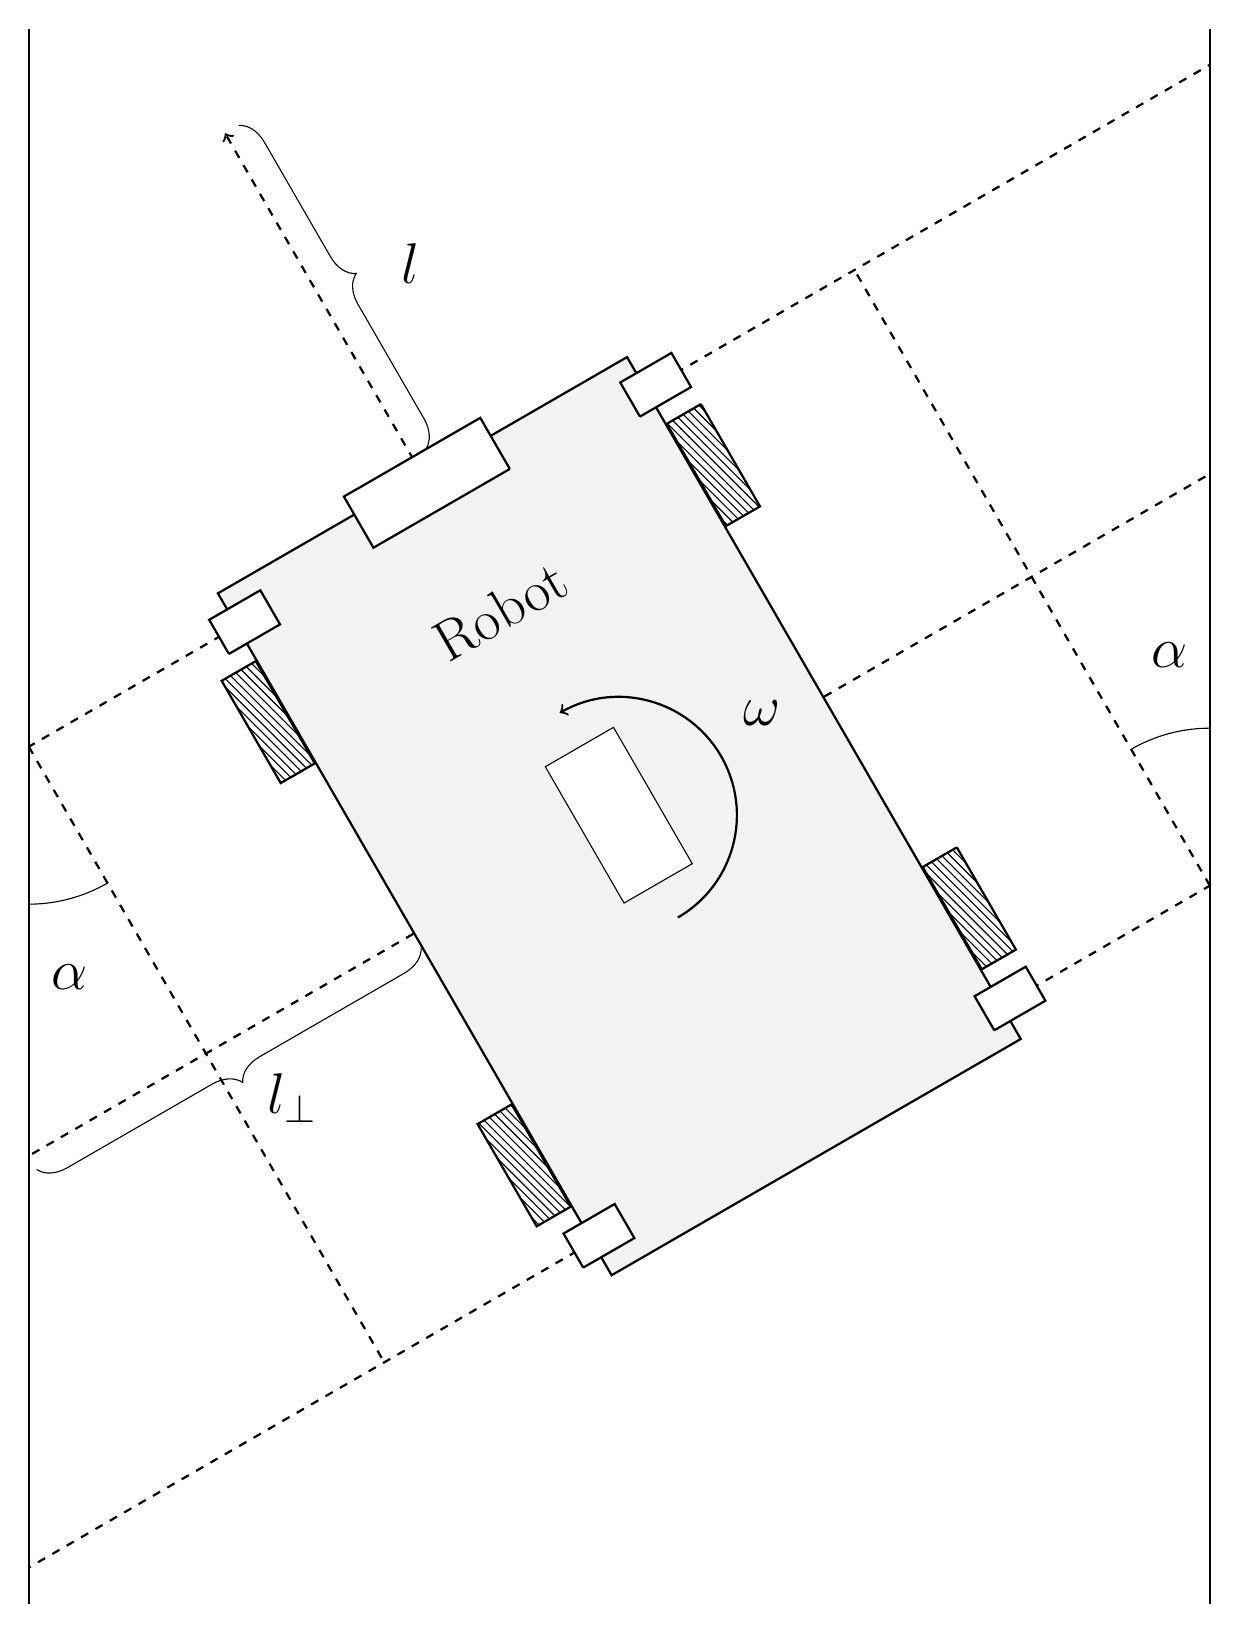
\begin{tikzpicture}[scale=1]
		
		%Sides
		\path [name path=left, draw=black,thick] (0,0) -- (0,20);
		\path [name path=right, draw=black,thick] (15,0) -- (15,20);	

		%Robot
		\node (robot) at (7.5,10) [draw, thick, minimum width=6cm, minimum height=10cm,align=center,rotate=30,fill=gray!10] {};
		\node [rotate=30] at ($(robot.north) + (-60:2cm)$) {\huge Robot};
		\node [rotate=30,minimum width=1cm, minimum height=2cm, fill=white,draw=black] at ($(robot.north) + (-60:5cm)$) {};
		\coordinate (start1) at ($(robot.north west) + (-60:.5cm)$);
		\coordinate (start2) at ($(robot.south west) + (120:.5cm)$);
		\coordinate (start3) at ($(robot.north east) + (-60:.5cm)$);
		\coordinate (start4) at ($(robot.south east) + (120:.5cm)$);
		
		\coordinate (middle1) at ($(robot.north west) + (-60:5cm)$);
		\coordinate (middle2) at ($(robot.north east) + (-60:5cm)$);
		
		\path [name path=path1,overlay,rotate=30] (start1) -- +(-20cm,0cm);
		\path [name path=path2,overlay,rotate=30] (start2) -- +(-20cm,0cm);
		\path [name path=path3,overlay,rotate=30] (start3) -- +(20cm,0cm);
		\path [name path=path4,overlay,rotate=30] (start4) -- +(20cm,0cm);
		
		\path [name path=middlePath1,overlay,rotate = 30] (middle1) -- +(-20cm,0cm);
		\path [name path=middlePath2,overlay,rotate = 30] (middle2) -- +(20cm, 0cm);
		
		\path [name path=left1, name intersections={of=path1 and left, by=x1},thick, draw=black,dashed] (start1) -- (x1);
		\path [name path=left2, name intersections={of=path2 and left, by=x2},thick, draw=black,dashed] (start2) -- (x2);
		\path [name path=right1, name intersections={of=path3 and right, by=x3},thick, draw=black,dashed] (start3) -- (x3);
		\path [name path=right2, name intersections={of=path4 and right, by=x4},thick, draw=black,dashed] (start4) -- (x4);
		
		\path [name path=int1, name intersections={of=left and middlePath1, by=m1}, thick, draw=black, dashed] (middle1) -- (m1);
		\path [name path=int2, name intersections={of=right and middlePath2, by=m2}, thick, draw=black, dashed] (middle2) -- (m2);
		
		\path [name path=kat1,overlay] (x1) -- +(-60:20cm);
		\path [name path=kat2,overlay] (x4) -- +(120:20cm);
		
		\path [name intersections={of= kat1 and left2, by=x5}, thick, draw=black,dashed] (x1) -- (x5);
		\draw ($(x1) - (0,2cm)$) arc [start angle=-90, end angle=-60, radius=2cm,thick] node [midway, yshift=-1cm] {\huge $\alpha$};
		
		\path [name intersections={of= kat2 and right1, by=x6}, thick, draw=black,dashed] (x4) -- (x6);
		\draw ($(x4) + (0,2cm)$) arc [start angle=-270, end angle=-240, radius=2cm,thick] node [midway, yshift=1cm] {\huge $\alpha$};
		\draw[thick, draw=black, ->,dashed] (robot.north) --+(120:5cm);
		
		\draw [thick, draw=black, ->] ($(robot.north) + (-60:6.5cm)$) arc [start angle=300, end angle=480, radius=1.5cm, thick] node[right=2.2cm] {\huge $\omega$};
		
		\draw [thick, fill=white, rotate=0] ($(robot.north west) + (-60:.75cm) + (-150:0.25cm)$) -- ($(robot.north west) + (-60:.75cm) + (-150:-0.5cm)$) -- ($(robot.north west) + (-60:0.25cm) + (-150:-0.5cm)$) -- ($(robot.north west) + (-60:0.25cm) + (-150:0.25cm)$) -- ($(robot.north west) + (-60:0.75cm) + (-150:0.25cm)$);
		
		\draw [thick, fill=white, rotate=0] ($(robot.north west) + (-60:9.75cm) + (-150:0.25cm)$) -- ($(robot.north west) + (-60:9.75cm) + (-150:-0.5cm)$) -- ($(robot.north west) + (-60:9.25cm) + (-150:-0.5cm)$) -- ($(robot.north west) + (-60:9.25cm) + (-150:0.25cm)$) -- ($(robot.north west) + (-60:9.75cm) + (-150:0.25cm)$);
		
		\draw [thick, fill=white, rotate=0] ($(robot.north east) + (-60:.75cm) + (-150:0.25cm)$) -- ($(robot.north east) + (-60:.75cm) + (-150:-0.5cm)$) -- ($(robot.north east) + (-60:0.25cm) + (-150:-0.5cm)$) -- ($(robot.north east) + (-60:0.25cm) + (-150:0.25cm)$) -- ($(robot.north east) + (-60:0.75cm) + (-150:0.25cm)$);
		
		\draw [thick, fill=white, rotate=0] ($(robot.north east) + (-60:9.75cm) + (-150:0.25cm)$) -- ($(robot.north east) + (-60:9.75cm) + (-150:-0.5cm)$) -- ($(robot.north east) + (-60:9.25cm) + (-150:-0.5cm)$) -- ($(robot.north east) + (-60:9.25cm) + (-150:0.25cm)$) -- ($(robot.north east) + (-60:9.75cm) + (-150:0.25cm)$);
		
		\draw [thick, pattern=north west lines, pattern color=black] ($(robot.north west) + (-60:1cm)$) -- ++(30:-.5) -- ++(120:-1.5cm) -- ++(30:.5) -- +(-60:-1.5);
		\draw [thick, pattern=north west lines, pattern color=black] ($(robot.north west) + (-60:7.5cm)$) -- ++(30:-.5) -- ++(120:-1.5cm) -- ++(30:.5) -- +(-60:-1.5);
		
		\draw [thick, pattern=north west lines, pattern color=black] ($(robot.north east) + (-60:1cm) + (30:.5cm)$) -- ++(30:-.5) -- ++(120:-1.5cm) -- ++(30:.5) -- +(-60:-1.5);
		\draw [thick, pattern=north west lines, pattern color=black] ($(robot.north east) + (-60:7.5cm) + (30:.5cm)$) -- ++(30:-.5) -- ++(120:-1.5cm) -- ++(30:.5) -- +(-60:-1.5);
		
		\draw [thick, fill=white] ($(robot.north) + (30:1cm) + (-60:0.5cm)$) --++(120:0.75cm) --++(210:2cm) --++(-60:0.75cm) --++(30:2cm);
		
		\draw [decorate,decoration={brace,amplitude=10pt},xshift=-10pt,yshift=0pt] ($(robot.north) + (120:5cm) + (30:0.2cm)$) -- +(120:-4.75cm) node [black,midway,xshift=1cm,yshift=0.3cm] {\huge $l$};
		
		\draw [decorate,decoration={brace,amplitude=10pt},xshift=-10pt,yshift=5pt] ($(middle1) +(-60:.2cm)$) -- ($(m1) +(-60:.2cm)$) node [black,midway,xshift=.8cm,yshift=-.5cm] {\huge $l_{\perp}$};
		
	\end{tikzpicture}
	
\end{document}